The approach takes place in three discrete phases: \textit{data collecton}, \textit{data processing} and \textit{analysis}, as summarized
by figure \ref{pipeline}.

\ \\ 
\raggedbottom
\begin{tabular}{@{}cc}
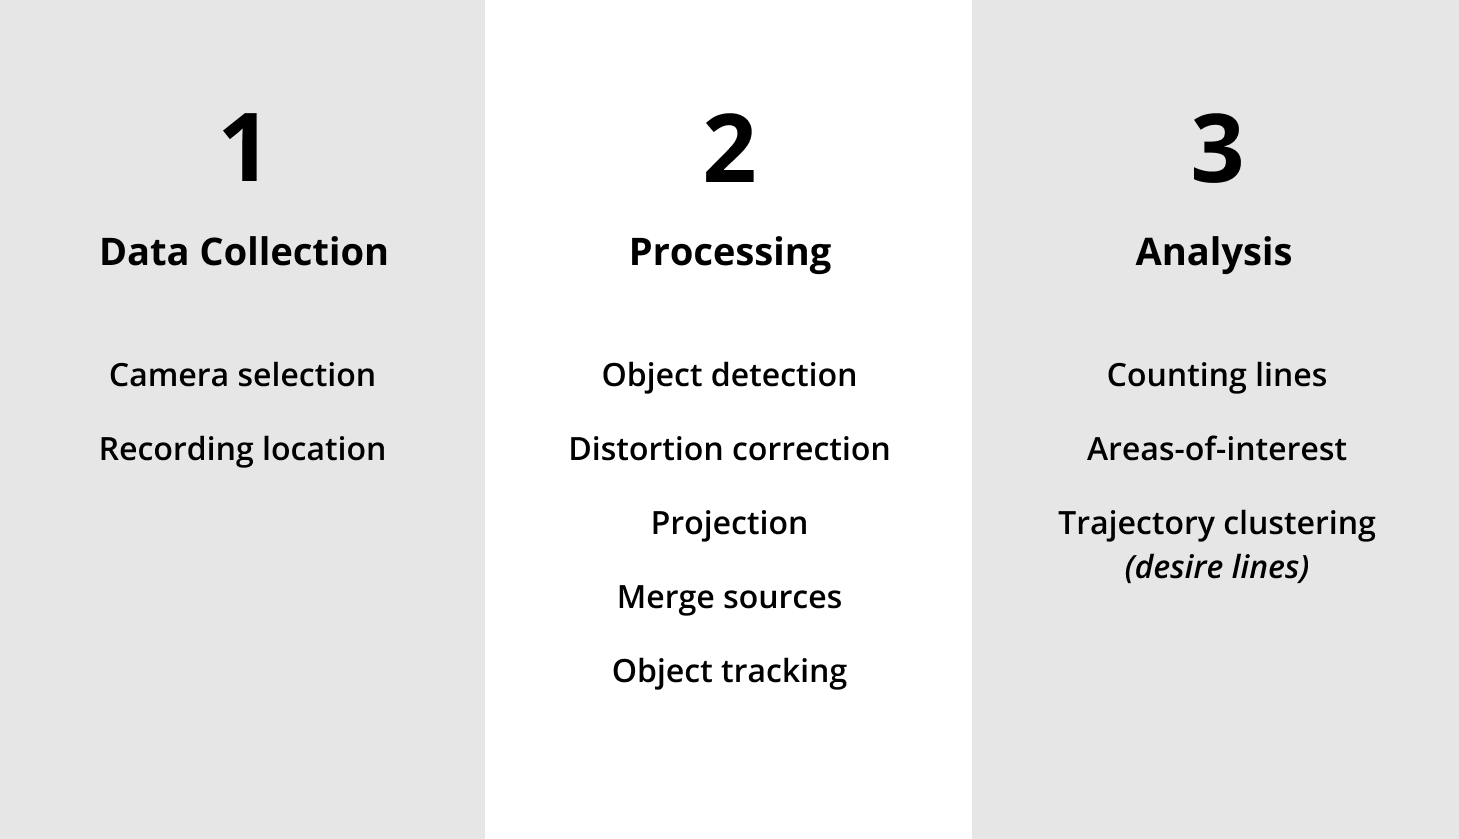
\includegraphics[width=1.0\columnwidth]{pipeline} 
\end{tabular}
\captionof{figure}{Overview of data pipeline} 
\label{pipeline}

\subsection{Data Collection}
\ \\ 
\noindent
\begin{tabular}{@{}cc}
\includegraphics[width=1.0\columnwidth]{dybbølsbro}
\end{tabular}
\captionof{figure}{Dybbølsbro/Ingerslevgade intersection \\ (\textit{Københavns Kommune})} 
\label{intersection_overview}
\

Our work is centered around the Dybbølsbro / Ingerslevgade intersection south-east of Copenhagen
city center. The intersection faces several challenges, producing \textit{"conflicts, unsafe situations, illegal 
road user behavior and great dissatisfaction among road users at the intersection"} (\cite{CPHpost_2021}).
From the south the intersection connects to the Dybbølsbro bridge, which features a bi-directional cycle path, two
lanes for vehicle traffic as well as pedestrians from the nearby train station. 
This is an unusual setup in Copenhagen, as most streets feature unidirectional cycle paths 
following vehicle traffic. Therefore, south-bound cyclists coming from the north (Skelbækgade) have to perform a two-phase 
turn to continue over the bridge. Firstly by heading straight over the intersection, but then having to stop and perform a left turn to 
continue. This leads to high congestion at the south-west corner of the intersection with many cyclists looking for a shortcut across. 
Due to its issues and size as well as previous analysis done on the intersection, we found it to be a good baseline for experimentation.

\subsubsection{Recording Location}
There are two considerations to take into account when recording an intersection for video analysis.
\ \\

\textbf{intersection size} \\
The size of the intersection will determine the camera setup needed. Larger intersections require a two-camera setup as detailed, 
but this might not be optimal for intersections much larger than the Dybbølsbro intersection. 
Initially we used a single camera setup, but found that while we had a good view of the entire intersection, 
we lost tracking data when the view of the cyclist on the opposite side on the intersection where obstructed by vehicles.
\ \\

\textbf{Camera mounting points} \\
We tried three different mounting locations as show by the red and purple circles in figure \ref{intersection_overview}. 
We faced several difficulties with camera mounting at the intersection, including camera stability, 
obstructions of the camera view, and the height of the mounting positions. 
With some of our camera mounts, stability was impacted by wind and thus the camera was swaying, resulting in skewed detections later on.
To cover the entire intersection with adequate coverage, we selected a two-camera setup on opposite sides of the intersection.

\subsubsection{Camera setup}
Any camera device with an adequate field-of-view (FOV) to capture the intersection, records in HD (1280×720 resolution) at a constant 
frame rate (at least 10FPS), and allows remote viewing of its viewfinder will suffice. 
However, having tested a Raspberry Pi recording setup (including a camera module, external battery, and an LCD touch screen), 
we would not recommend a self-built recording setup. Although the Raspberry Pi setup meets the above-mentioned technical requirements, 
the challenges lie in the usability of such a setup. 
It introduces unnecessary complexities by having to manually assemble the hardware and install necessary software, as well as 
having surety of its operation in the field.
Alternative devices optimized for video recording such as mobile phones or action cameras are more suitable.
These devices typically offer methods of remotely controlling and viewing their software interface from 
another device such as a PC or smartphone, including the viewfinder. 
This is useful when mounting the camera and adjusting its position to get a good view of the intersection. 
While also possible with a Raspberry Pi, it is less stable in comparison to using smartphones or action cameras.
Hence, we chose to use smartphones for recording, namely an \textit{LG G6} and a \textit{Samsung Galaxy S7 Edge}.

% Along with meeting the basic requirements they also have Ingress Protection ratings, 
% commonly referred to as waterproofing. This should be considered if rain is a possibility.
\ \\

% Given a recording location, we can use (eq. \ref{eq:1}) to calculate the FOV a camera needs to capture an intersection.
% If $\theta > FOV$, then the FOV is too small.
% \color{red}
% Note: Label images and make them more understandable.
% \color{black}

% \begin{equation}
%     \theta = tan^-1(\frac{\frac{width}{2}}{adjacent}) * 2\label{eq:1}
%   \end{equation}

% \ \\ 
% \raggedbottom
% \begin{tabular}{@{}cc}
% 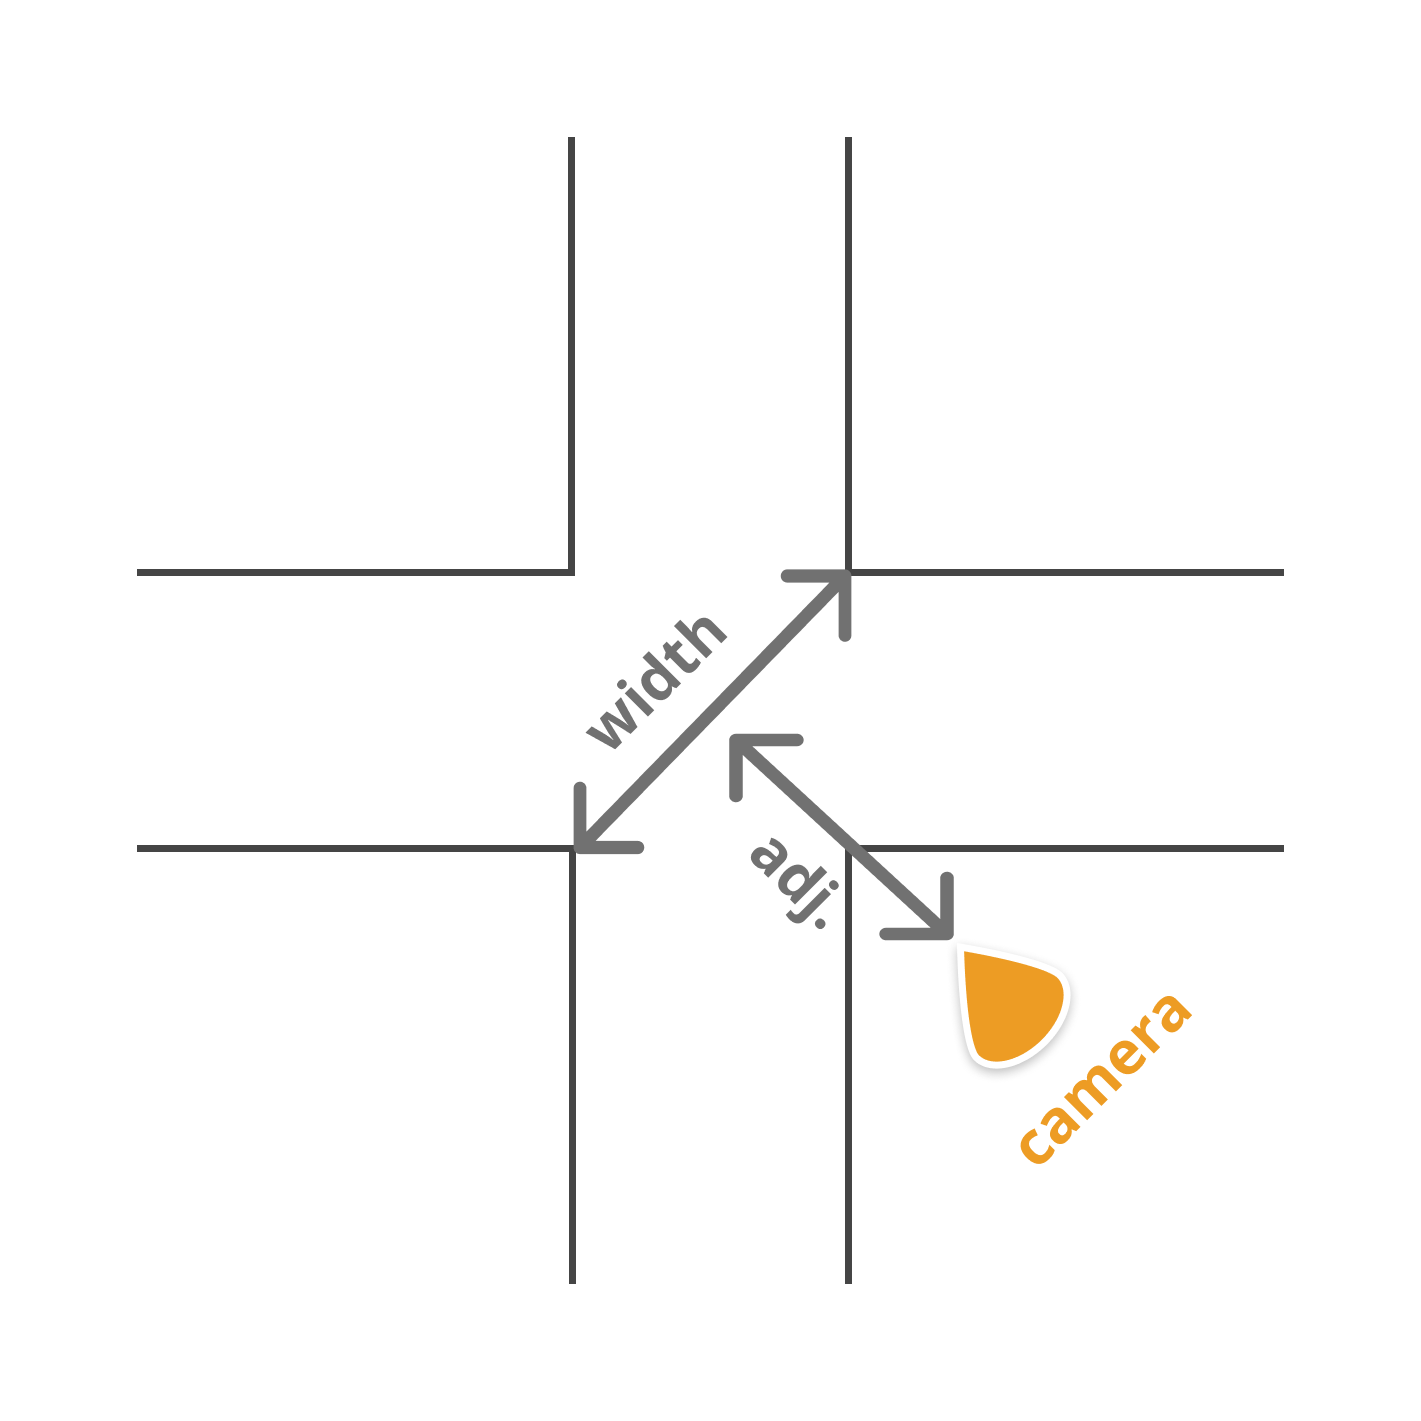
\includegraphics[width=1.0\columnwidth]{location} 
% \end{tabular}
% \captionof{figure}{Camera location}
% \label{Camera location}
% \

% Battery life and storage capacity should also be considered depending on the amount of intended recording. 
% With regards to storage, a good estimate for video size would be 149MB per 1 min of FullHD (1920*1080) at 30FPS. Storage should be selected
% with the intended amount of recording time.

\ \\ 
\raggedbottom
\begin{tabular}{@{}cc}
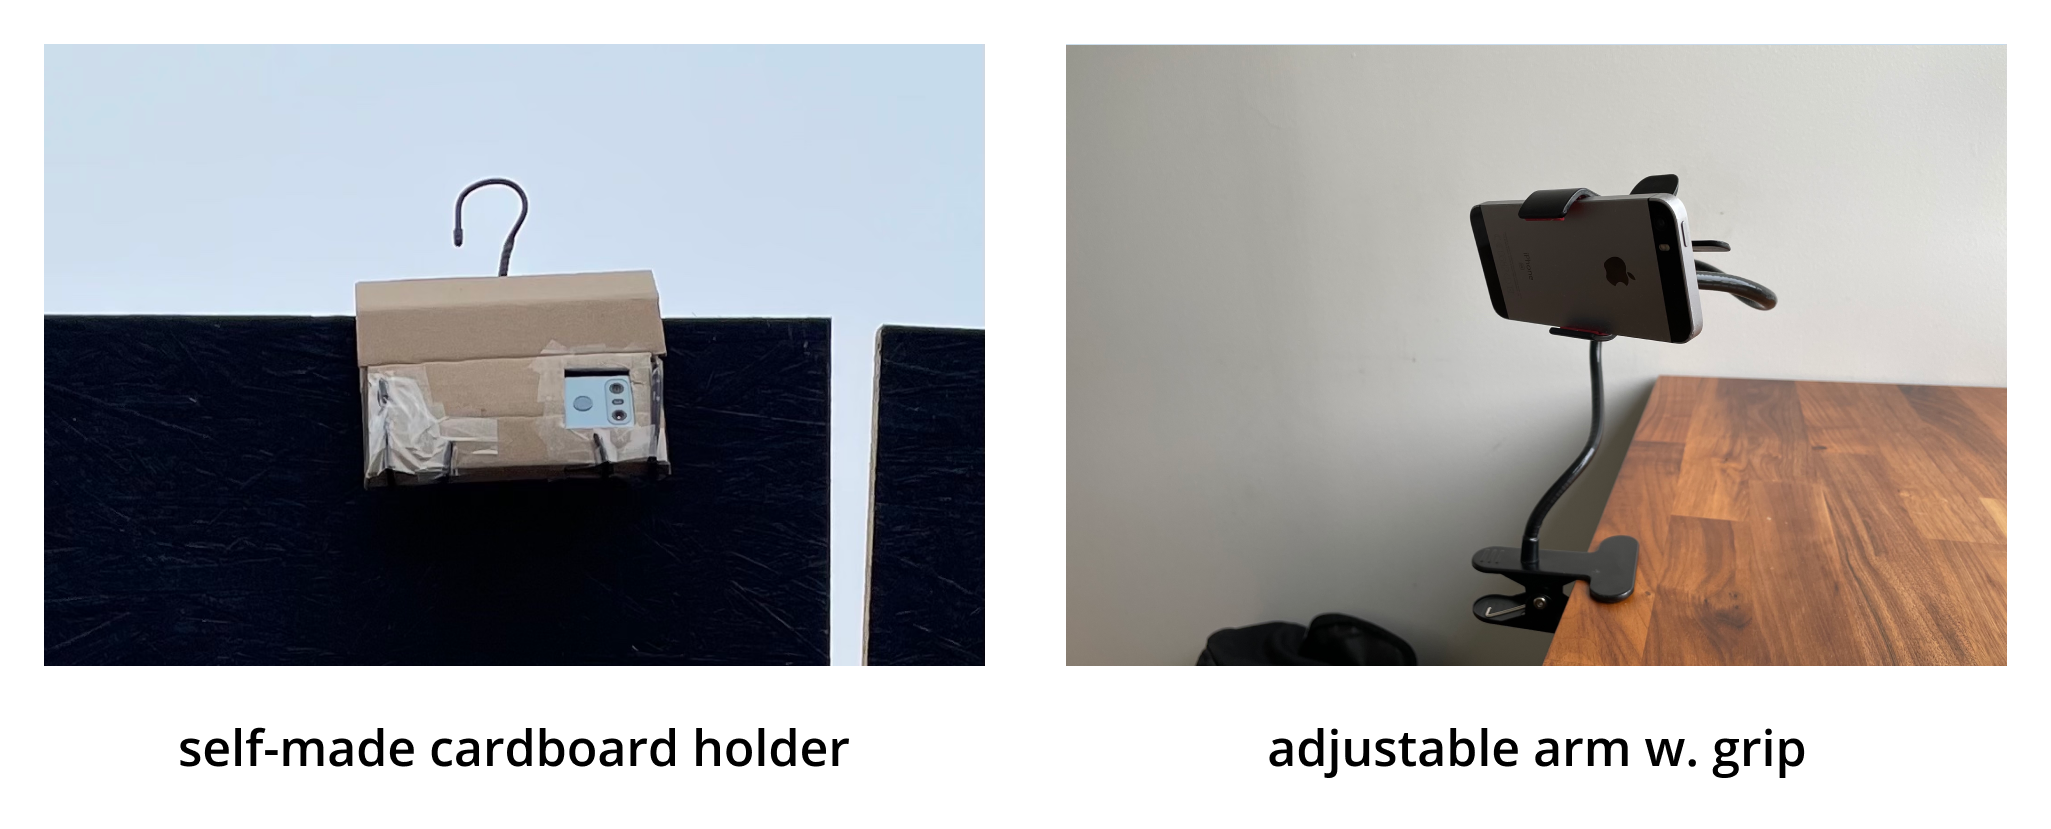
\includegraphics[width=1.0\columnwidth]{contraptions}
\end{tabular}
\captionof{figure}{Camera mounts} 
\label{camera_mouns}
\

We used two different methods of mounting cameras at the intersection. One includes a flexible arm which can be clammed onto infrastructure such as light poles.
The second mounting solution was a self-built holder made out of cardboard and a hook, allowing us to easily mount it at high spots using a long extension rod.
Selecting an appropriate mounting height is a trade-off between maximizing the captured area of the intersection and having a frontal view of traffic.
We aimed to always have cameras mounted at least 3-4 meters above ground.

\subsection{Data Processing}
\ \\ 

\color{red}
\raggedbottom
\begin{tabular}{@{}cc}
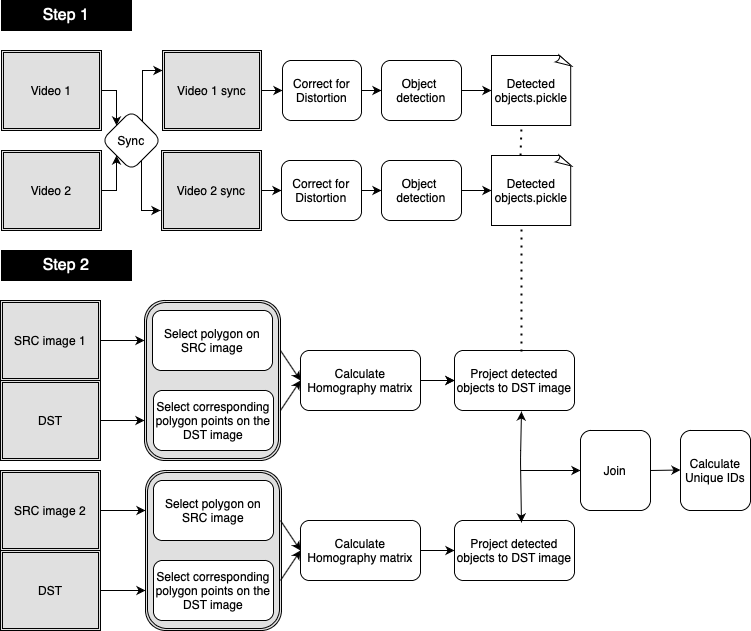
\includegraphics[width=1.0\columnwidth]{data_flow.png} 
\end{tabular}
\captionof{figure}{Data Pipeline}
\label{data}
\raggedbottom
\color{black}

\subsubsection{Video Syncing}
An important preprocessing step is to cut the different video soucres to the same time stamp.
Should the video have different frame rates or resolutions then these should be processed to match.

\subsubsection{Camera calibration}
Cameras often suffer from optical aberration where straight lines appear bent, especially noticable in the edges of an image. 
This can be observed on wide-angle camera lenses such as on the LG G6 we used.
The specific type is \textit{positive radial distortion} as shown in figure \ref{distortion_types}, with lines curving outwards in a barrel shape.
These aberrations are a result of the curved shape of the camera lens.
\ \\ 

\raggedbottom
\begin{tabular}{@{}cc}
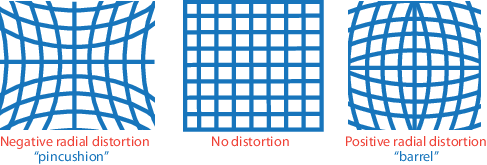
\includegraphics[width=1.0\columnwidth]{calibration_radial_distortion} 
\end{tabular}
\captionof{figure}{Types of lens distortion}
\label{distortion_types}
\

There is also a possibility of further distortion if the camera sensor and the lens are not parallel, also known as \textit{tangential distortion}.
Ideally, there should be no radial nor tangential distortion.
\ \\
It became apparent when merging data from multiple camera sources that lens distortion had an effect on the alignment of data points.
This is shown in figure \ref{joined_distortion}, Before Calibration.

\begin{figure}[h]
  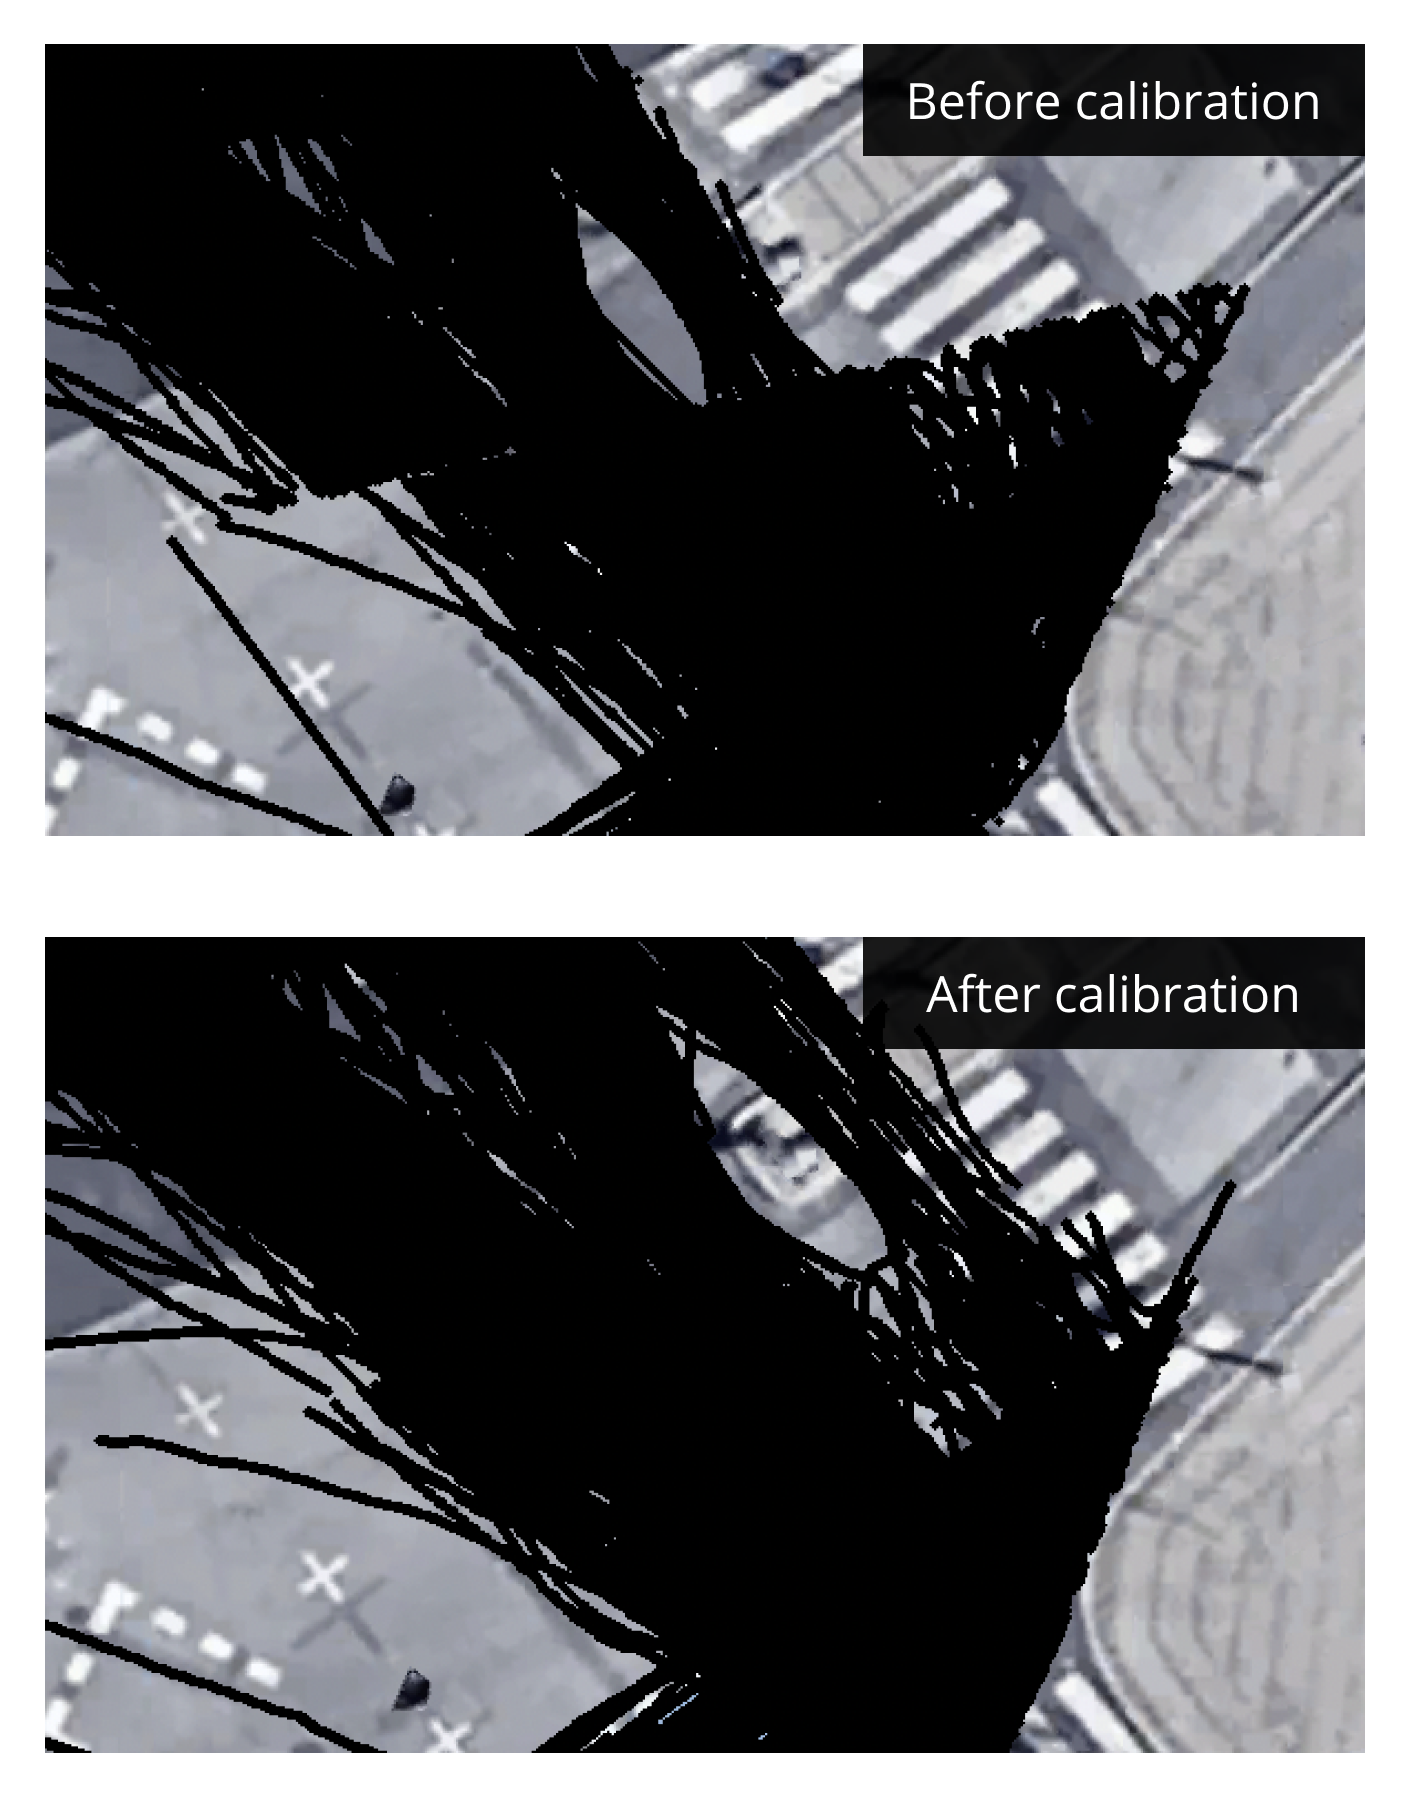
\includegraphics[scale=0.6]{calibration.png}
  \centering 
  \end{figure}
  \captionof{figure}{Distortion}
  \label{joined_distortion}
\ \\

To correct for teh distortion we make use of OpenCVs (\cite{noauthor_opencv/opencv_2021}) camera calibration toolbox.

In order to correct for distortion, we need to find the camera matrix and distortion coefficients. To do this we used the calibrate script provided with OpenCV,
passing several snapshots of a calibration object with the device to be calibrated. The calibration object being a black-white chessboard pattern.
We passed 20+ sample images of the calibration object in different orientations, angles and positions in the frame. OpenCV processes the pictures and
returns a camera matrix and the distortion coefficients, used for correcting the distortion of the frames.
\ \\

\subsubsection{Object Detection}
Object detection is the most important factor to consider, it is the key component in making this method work.
\ \\

We found that our offline OpenDataCam setup using an Nvidia Jetson NX setup worked well for detecting cars but didn't perform well on cyclists. 
We, therefore, implemented our object detection setup using
YOLOv5. YOLOv5 showed a good improvement on cyclists.
\ \\ 
Predicted objects are represented as bounding boxes with the output being represented as $[[frame id][xmin][ymin][xmax][ymax][confidence]]$

\subsubsection{Projection}
To achieve the "birds-eye view" of the intersection, we needed to explore methods of 
transforming the data from the camera views.  
\ \\
A homography matrix is a transformation matrix between two planes \cite{hartley_zisserman_2004}. It 
can be used to perform a perspective transformation of a plane from a source image $P(x_r, y_r)$ onto 
a plane on a destination image $Q(x_i, y_i)$.
The source image in our case is the plane of the road surface from the recorded videos at the intersection 
to the road surface from an aerial view of the same intersection. 
This will allow us to transform and plot the cyclist movements onto an aerial photograph of the intersection.
\ \\ 

\noindent
\begin{tabular}{@{}cc}
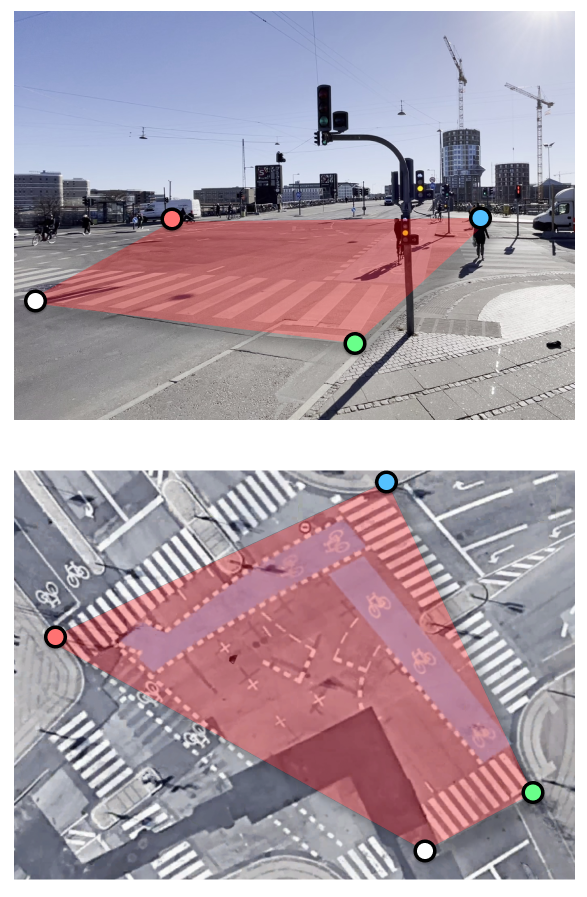
\includegraphics[width=1.0\columnwidth]{projection_figure} 
\end{tabular}
\captionof{figure}{Projection - ground control points}
\label{projection_figure}
\

To calculate the homography matrix, we need to solve the for the system of linear equations, $P = HQ$,
\ \\
$P$ being points in a polygon on the source image, $Q$ the corresponding polygon on the destination image $H$ being the homography matrix.
\begin{align}
\label{eq:3}
  \begin{bmatrix}
    x_{i} \\
    y_{i} \\
    z_{i} \\
  \end{bmatrix}
  &= \begin{bmatrix}
      h_1 & h_2 & h_3 \\
      h_4 & h_5 & h_6 \\
      h_7 & h_8 & h_9 \\
  \end{bmatrix}
  \begin{bmatrix}
    x_{r} \\
    y_{r} \\
    z_{r} \\
  \end{bmatrix}
\end{align}
\ \\

Before we can project the cyclist onto an aerial view, we first need to calculate the 2D coordinates of their contact points with the road surface.
Given the below equation, we can calculate the contact points.

$$x = xmin + \frac{(xmax - xmin)}{2}$$
$$y = ymin$$

Using the homography matrix, we can now project the contact points $(x, y)$ of the cyclist onto the destination
image. This is achieved by applying $z$ to each point as a constant to create $Q(x_i, y_i, 1)$ and then we multiply it by the homography matrix. 

\subsubsection{Merging Sources}
As we are using multiple video sources, there will be an overlap of the detected cyclists. 
That is, the trajectory of the same cyclist will be captured by multiple cameras for certain areas. 
To merge the trajectories from the video sources, we take a naive approach. As the cameras are set up on
opposite sides of the intersection, we simply cut the video sources in half along the mid-point between
the two cameras along the intersection to join them.

\ \\ 
\noindent
\begin{tabular}{@{}cc}
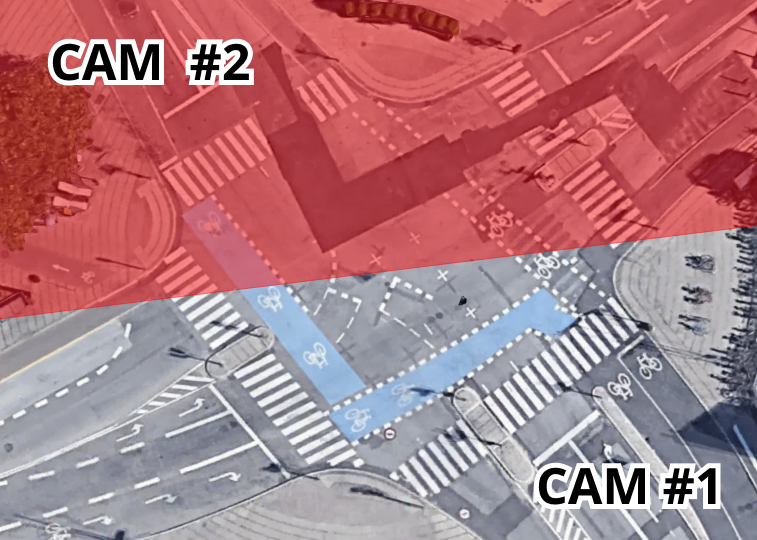
\includegraphics[width=1.0\columnwidth]{slice} 
\end{tabular}
\captionof{figure}{Cutting of video sources}
\label{slice}
\

\subsubsection{Tracking}

In order to connect detections into trajectories of individual cyclist, we apply 
the \href{https://github.com/abewley/sort}{SORT algorithm}, \textit{simple online and real-time tracking}, as initially described in (\cite{Bewley2016_sort}). 
SORT aims to address multiple object tracking (MOT) where objects across frames needs to be connected. 
\ \\ 

SORT uses a Kalman Filter to predict bounding boxes. A predicted bounding box \textit{A} and a Bounding box \textit{B} from 
frame t+1 are compared using their Intersection over Union (IOU). IOU is calculated by dividing the area of overlap between the 
bounding boxes by the area of union of the bounding boxes. If the IOU is above a certain threshold, the two points are connected as the same object.
\ \\ 

In our implementation we define arbitrary bounding boxes around the center point of the projected detections; 
we used a 10x10 pixel bounding box. This is a result of the plane of the bounding boxes from the object detection is on
a different plane to that of the roads surface.

\subsection{Data Exploration}

\subsubsection{Web app}
To interact with the tools implemented, we created a simple web application using the \href{https://plotly.com/dash/}{Dash library} for Python. 
Its main components consist of a satellite/aerial view of the chosen intersection with the trajectories of cyclists plotted as short-lived tracks. 
One can then scrub through time by either explicitly referencing to a timestamp or frame, using a slider or jump in set increments.
Below the aerial view is a set of image viewers showing the current frame from all the cameras with markers around selected cyclists.

\ \\ 
\raggedbottom
\begin{tabular}{@{}cc}
\includegraphics[width=1.0\columnwidth]{webapp} 
\end{tabular}
\captionof{figure}{Web application}
\label{webapp}
\

To gain insight into specific areas of the intersection, one can filter observations by drawing a mask on the aerial view. 
When an area is selected, all cyclists passing it will be listed in a side panel, from which one can jump directly to the matching timestamp.
\
Counting lines (as also found in OpenDataCam) are also implemented, giving the user the ability to immediately see the number of 
cylists passing certain parts of the intersection in either direction.
\ \\

\textbf{Future work} \\
Currently the data pre-proccesing is not part of the application, thereby functioning more as a \textit{proof of concept}.
It would be relatively easy to connect the data processing pipeline to the web interface, thus simply making the user 
select video sources, map the \textit{ground control points} (for aerial projection) and potentially tweaking other hyper-parameters. 

\subsubsection{Rainbow Tracks}

\ \\ 
\noindent
\begin{tabular}{@{}cc}
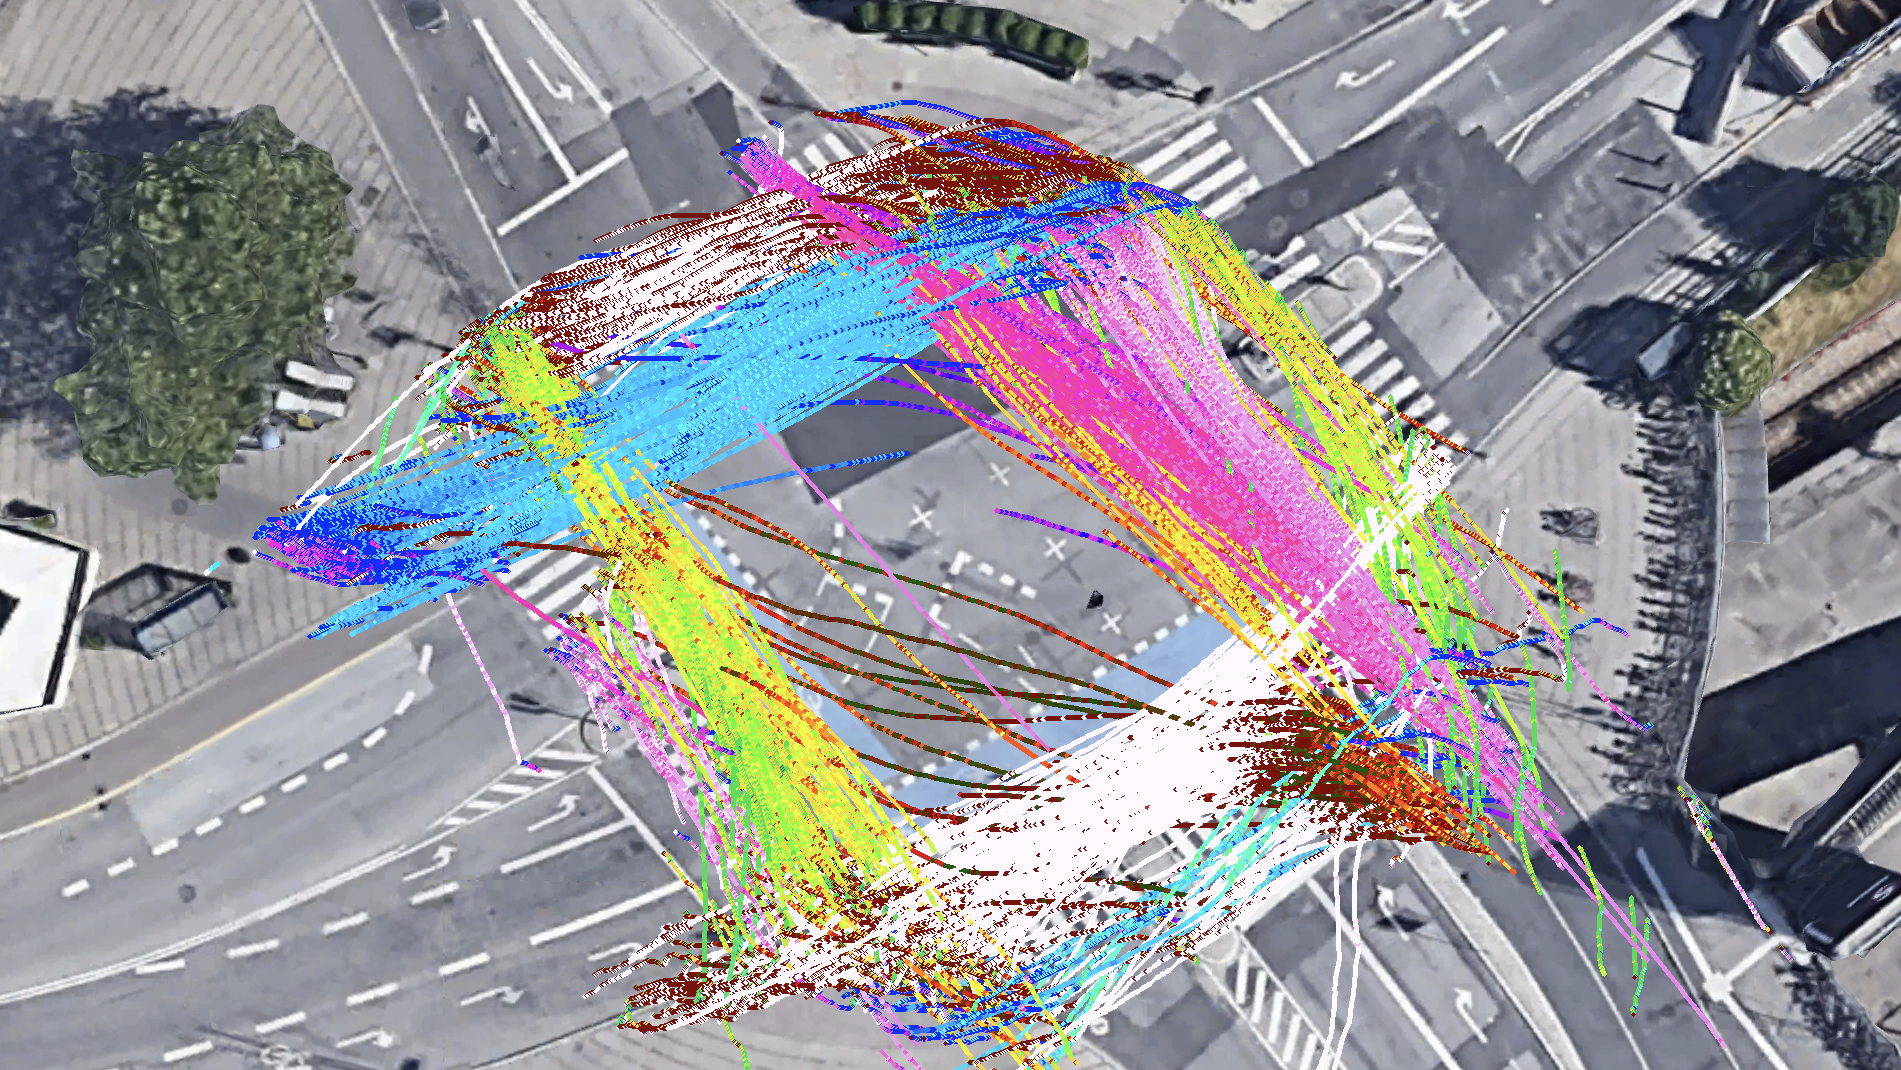
\includegraphics[width=1.0\columnwidth]{rainbow.png} 
\end{tabular}
\captionof{figure}{Rainbow Tracks}
\label{Rainbow}
\

To find aggregated desire lines from the data we took an approach which we call "Rainbow tracks". 
This involves coloring tracks by the bearing between consecutive points in each trajectory. 
After calculating the bearing, we then get a color from a gradient color wheel. 
This approach has the added benefit of encoding direction into each track.
\ \\ 

% \begin{equation}
%   UniqueID_i = [(x_1, y_1)...(x_a+1, y_a+1)]\label{eq:3}
% \end{equation}

